\section{Stream Programming Model}

\begin{figure}[t]
\begin{center}
%\vspace{-24pt}
% \framebox{
 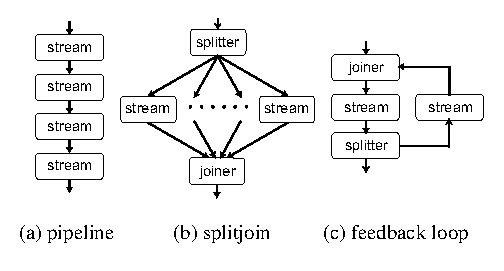
\includegraphics[scale=1, angle=0]{./constructs-eg.eps}
%}
% \vspace{-6pt}
% \nocaptionrule
 \caption{Examples of hierarchical streams.}
 \label{fig:containers}
\end{center}
\end{figure}

There are are a number of stream-oriented languages drawing from
domains such as functional, dataflow, CSP and synchronous
programming~\cite{survey97}. We assume an architecture-independent
programming language for high-performance stream programming. The
language expresses computation as a structured hierarchical graph of
{\it actors} connected by FIFO communication channels. Actors are
referred to as {\it filters} in some languages such as
StreamIt~\cite{streamitcc,streamit-lang-spec}. Filters use explicit
data channels for all communication. Each filter contains a {\tt work}
function that executes a single step of the filter.  From within {\tt
work}, filters can {\it push} items onto the output channel, {\it pop}
items from the input channel, or {\it peek} at an input item without
removing it from the channel. Peeking exposes data parallelism in
sliding-window filters (e.g., FIR filters) and are conceptually
equivalent to filters that maintain some internal state.

We assume there are three fundamental primites for hierarchically
composing filters into larger stream graphs.  A {\it pipeline}
connects streams sequentially. A {\it splitjoin} specifies
independent, parallel streams that diverge from a common {\it
splitter} and merge into a common {\it joiner}. The final hierarchical
primitive is a {\it feedbackloop} that provides a way to create cycles
in the graph. In practice, feedbackloops are rare and we do not
consider them in this paper.

\subsection{Execution of Stream Program}

An execution a stream program requires running all of the filters in
the stream graph in some order that satisfies the dependencies in the
graph. For example consider a simple pipeline consisting of three
filters $A\rightarrow B\rightarrow C$. Here $A\rightarrow B$ denotes a
FIFO connection between filters $A$ and $B$ such that $B$ pops data
pushed by $A$; and similarly for $B\rightarrow C$. A pull schedule for
$C$ is one that executes (fires) other nodes as few times as possible
for each firing of $C$. This is achieved by calculating the demand for
data items on the input channels of $C$, and then propagating the
demand back through the stream graph via pull scheduling of the
filters connected to $C$. Pull scheduling results in a fine-grained
interleaving of filter firings, and executes each node in the graph as
few times as possible for $C$ to fire a desired number of times.
Assuming that $A$ pushes one item and $B$ pops and pushes two items
per work function, the pull schedule for one $C$ firing requires two
firings of $A$ followed by one firing of $B$. A schedule implies
buffering requirements between filters, or in other words, it imposes
a minimum bound on the size of each FIFO between pairs of filters.

A stream program may be scheduled statically or dynamically. A static
schedule require some knowledge of the input and output rates of each
filter in the graph.

\subsection{Stateless and Stateful Filters}

A filter with no state...

A filter with state...